%
% ---------------------------------------------------
%
% Trabajo Fin de Grado:
% Author: Víctor Hernández Pérez 
% Correo: alu0100697032@ull.edu.es
% Capítulo: Descripción de la App
%
% ----------------------------------------------------
%

\cleardoublepage

\chapter{Descripción de la aplicación}
En este capítulo se presentarán las distintas actividades de la aplicación, comentando las características y que función tiene cada una de ellas.

Como paso previo a realizar el diseño de la aplicación, se investigaron otras 
apliaciones de carácter similar, con lo cual se han dedicado algunas secciones a este tema.

\section{Applicaciones universitarias}

Uno de los primeros pasos en la elaboración del trabajo fue elaborar un estudio comparativo de distintas aplicaciones universitarias para identificar cuáles eran las características que más se repetían entre ellas y evaluar si podrían formar parte de la aplicación final. 

El estudio se llevó a cabo con las aplicaciones de las universidades de: Murcia, 
Alicante, Valencia y de La Complutense de Madrid. Y se concluyó que las funcionalidades más usuales en este tipo de aplicaciones son:

\begin{itemize}
\item Disponer de un menú de opciones.
\item Autenticación del usuario.
\item Sección de noticias institucionales.
\item Sección de mapas para mostrar distintas ubicaciones de interés.
\end{itemize}

\section{AppTui}

Además se tubo como referencia la aplicación del Observatorio appTUI \cite{URL::appTUI} 
es una aplicación gratuita para smartphones 
que tiene como finalidad ayudar a los usuarios de la TUI a sacar el mayor partido de 
todas las ventajas y servicios de su tarjeta. 

La TUI se vincula a la aplicación mediante la lectura de un código QR asociado a cada tarjeta. 
A partir de ese momento el usuairo puede, de forma sencilla, cómoda y segura, acceder a la 
información de todos los servicios TUI de su universidad, con la ventaja de poder recibir además
todas las alertas recordando reservas realizadas, así como las novedades y, en general, toda 
la información necesaria para hacer más ágil la gestión académica y administrativa dentro de la Universidad.

\begin{figure}[h]
	\centering
	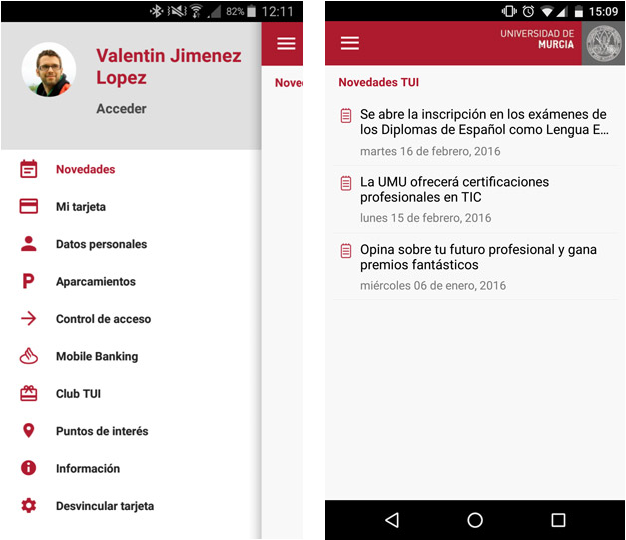
\includegraphics[width=0.6\columnwidth]{apptui.png}
	\caption{Vistas de appTUI}
	\label{fig:ejemplo}
\end{figure}


\section{Introducción a \App{}}

\App{} es una aplicación para dispositivos Android (App) para la Universidad de La Laguna 
que permite autenticación social por parte de los usuarios para obtener acceso a diferentes servicios, 
entre los cuales se encuentran:

\begin{itemize}
\item Sección de noticias.
\item Ubicación y descripción de ciertos puntos de interés de la universidad.
\item Reserva de pistas deportivas disponibles en la universidad.
\item Acceso a datos personales.
\end{itemize}


%%%%%%%%%%%%%%%%%%%%%%%%%%%%%%%%%%%%%%%%

\section{Actividades}

En este punto se describirán las distintas actividades de la aplicación, qué funcionalidad 
y carácterísticas tiene cada una. 

\subsection{Actividad de Login}

Es la actividad inicial de la aplicación, dónde el usuario se autentica, como paso previo 
a poder acceder al resto de la funcionalidad de la aplicación. 
\newline

Se emplea el protocolo \textit{Oauth} \cite{URL::Oauth} para la autenticación del usuario. 
Oauth permite autorización segura de una API para aplicaciones de escritorio, web y móviles. 
\newline

Se le da al usuario la opción de autenticarse a través de Facebook o Google. En ambos casos 
el usuario no tiene que realizar ninguna confirmación adicional para el acceso de la aplicación 
a los datos, dado que éstos a los que accede son de carácter público y cualquiera puede acceder a ellos. 

En caso de que en el dispositivo existan varias cuentas de Facebook o de Google se le permitirá al usuario
elegir cual de ellas quiere usar. También, en caso de que no tenga cuenta de Facebook autenticada en el dispositivo
móvil, se le pedirá introducir los datos de la misma para poder iniciar sesión satisfactoriamente.

\begin{figure}[h]
	\centering
	
\includegraphics[width=0.4\columnwidth]{login.png}
	\caption{Actividad de login}
	\label{fig:ejemplo}
\end{figure}

\subsection{Actividad principal}

Una vez el usuario se ha autenticado se muestra la actividad principal de la 
aplicación y se le da acceso al resto de funciones de la misma. Consta de una 
barra de acción en la parte superior y el contenido de la actividad, el cual es 
un fragmento que varía dependiendo de dónde se encuentre navegando el usuario. 

La barra de acción (en inglés Action Bar o App Bar) es uno de los elementos más
importantes en el diseño de las actividades de una aplicación, dado que, 
proporciona una estructura visual y elementos con los que el usuario puede 
interactuar de manera intuitiva. Esto permite al usuario un rápido entendimiento
del funcionamiento de la aplicación, lo que hace que tenga una buena experiencia 
en el uso de la misma.

Los elementos clave en la barra de acción son: 

\begin{itemize}
\item Un espacio dedicado para dar una identidad a la aplicación e indicar al
usuario la ubicación dentro de la misma.
\item Acceder a acciones relevantes de la aplicación, como por ejemplo la búsqueda.
\item Dar soporte al menú de navegación, pestañas o listas desplegables.
\end{itemize}

En el caso de esta aplicación, el menú de navegación consta de una cabecera y de
una serie de opciones que permiten al usuario moverse dentro de la aplicación. 

En la cabecera se muestra: 

\begin{itemize}
\item La foto de perfil del usuario.
\item El nombre de usuario y el correo electrónico de la cuenta.
\end{itemize}

Las opciones del menú de navegación son: 

\begin{itemize}
\item Sección de noticias de la institución.
\item Acceso a los datos personales del usuario.
\item Acceso al servicio de reservas.
\item Ubicación de ciertos puntos de interés de la universidad.
\end{itemize}

\begin{figure}[h]
	\centering
	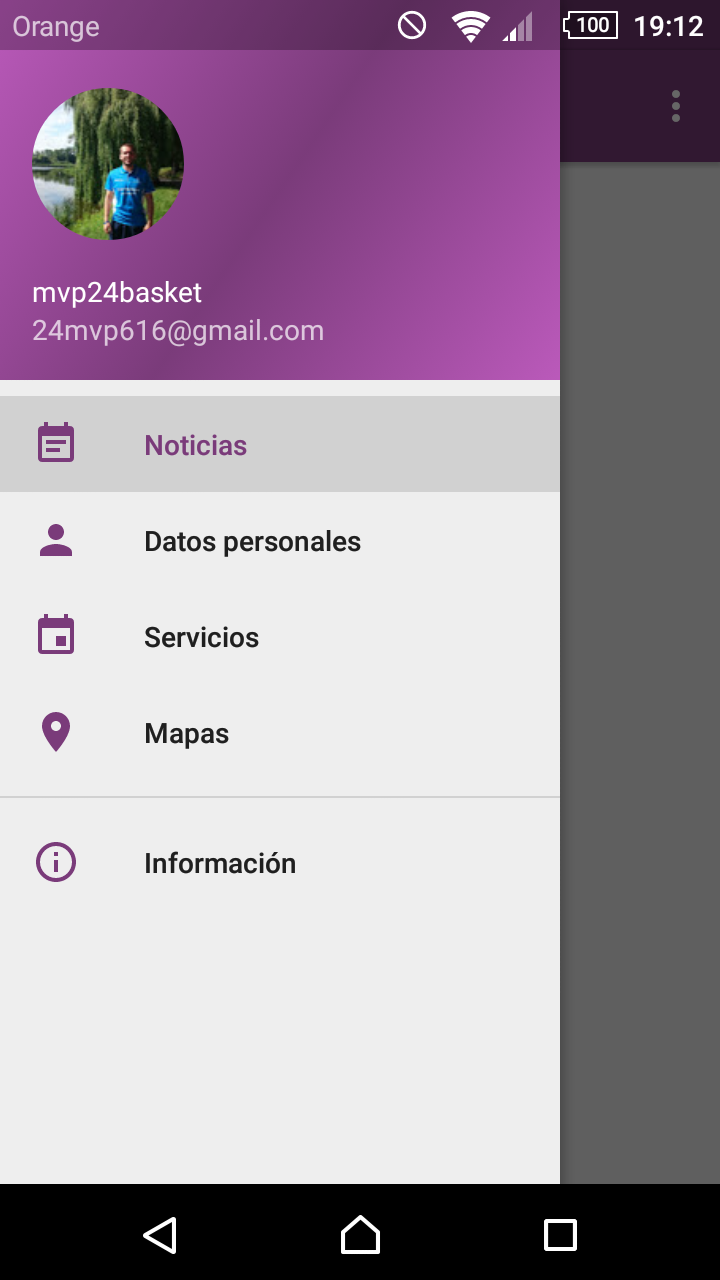
\includegraphics[width=0.4\columnwidth]{navview.png}
	\caption{Menú de navegación}
	\label{fig:ejemplo}
\end{figure}

En la barra de acción existe un botón de acción para la configuración que muestra 
una lista desplegable en la cual aparece una opción para cerrar sesión.
\newline

Para el contenido de esta actividad, se trabaja con fragmentos. Un fragmento 
representa una porción de la interfaz de usuario en una actividad. Se pueden 
combinar dentro de una misma actividad y reusar en diferentes actividades. Es una 
sección modular que tiene su propio ciclo de vida, recibe sus propios eventos y 
se pueden añadir o eliminar mientras la actividad está corriendo. Se podría 
definir como una sub actividad. 
\newpage

Podemos definir los siguientes fragmentos que serán utilizados como cuerpo de 
esta actividad: 

\begin{itemize}
\item El fragmento de noticias. En éste se muestra una lista de noticias de la 
institución. Se especifica: el título de la noticia, una descripción breve y la 
fecha de publicación de la misma.
\item El fragmento de información personal. Aquí se muestra toda la información 
del usuario referente a los servicios que se ofrecen en la aplicación. Dado que 
el único servicio que se ofrece, por ahora, es el de reserva de pistas, se muestra
información acerca de las reservas que ha hecho el usuario.
\item El fragmento de servicio. Aquí se muestra una lista de pistas que oferta 
la universidad para que puedan ser reservadas por el usuario.
\end{itemize}

\begin{figure}[h]
	\centering
	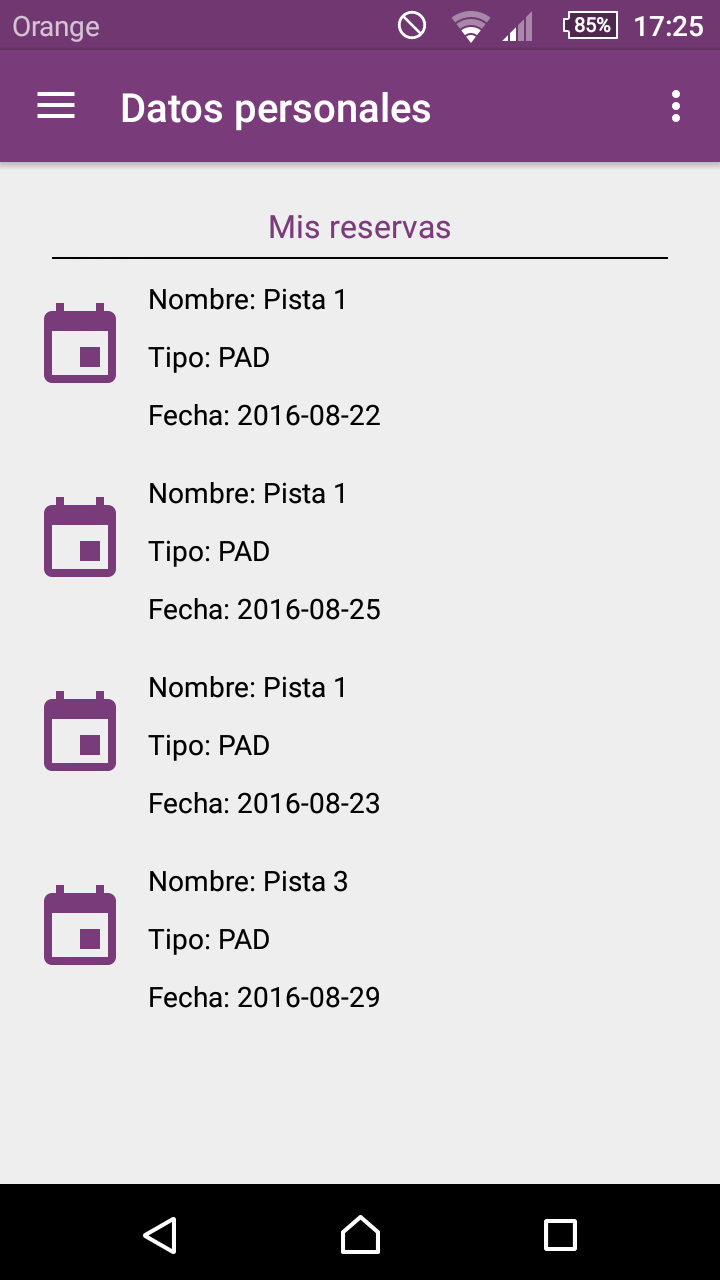
\includegraphics[width=0.35\columnwidth]{misServicios.png}
	\caption{Sección de Datos personales}
	\label{fig:ejemplo}
\end{figure}

\newpage

\subsection{Actividad de Logout}

Esta actividad se inicia cuando el usuario selecciona la opción de cerrar sesión
de la lista desplegable de la acción de configuración mencionado en el apartado 
anterior. 

La barra de acción cambia. La acción de configuración y el menú de navegación 
desaparecen para solo dar la opción al usuario de ir atrás o realizar la acción
de cierre de sesión. 

En el contenido de la actividad, se muestra: La foto de perfil del usuario y un
botón para hacer logout.

\begin{figure}[h]
	\centering
	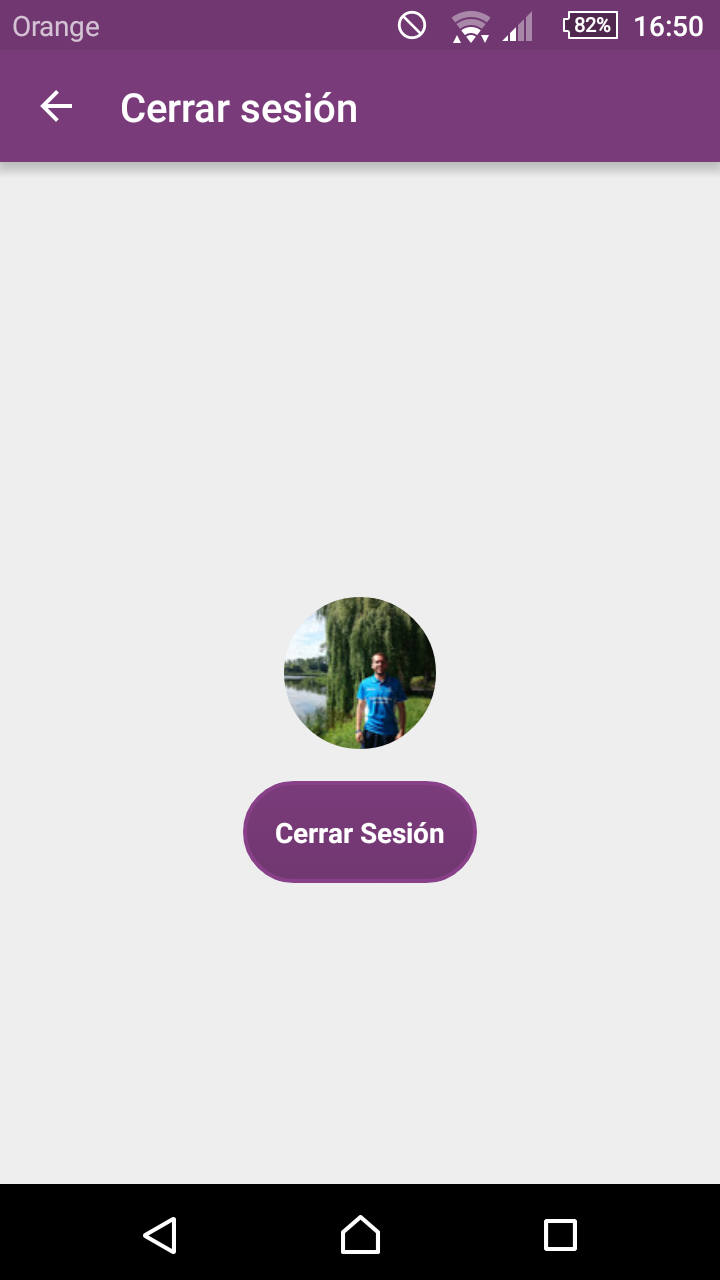
\includegraphics[width=0.4\columnwidth]{logout.png}
	\caption{Actividad de logout}
	\label{fig:ejemplo}
\end{figure}

\newpage

\subsection{Actividad de Leer Noticia}

En la Actividad Principal, descrita anteriormente, se mencionó que la sección 
de noticias estaba formada por una lista de noticias. Estas noticias se 
presentan de forma resumida al usuario para que, si le resulta de interés, pueda
interactuar con ella. 

Al tocar una noticia se inicia la actividad de Leer Noticia donde se muestra al usuario
toda la noticia para que pueda leerla al completo. 

La barra de acción cambia. La acción de configuración y el menú de navegación 
desaparecen para solo dar la opción al usuario de ir atrás.

\begin{figure}[h]
	\centering
	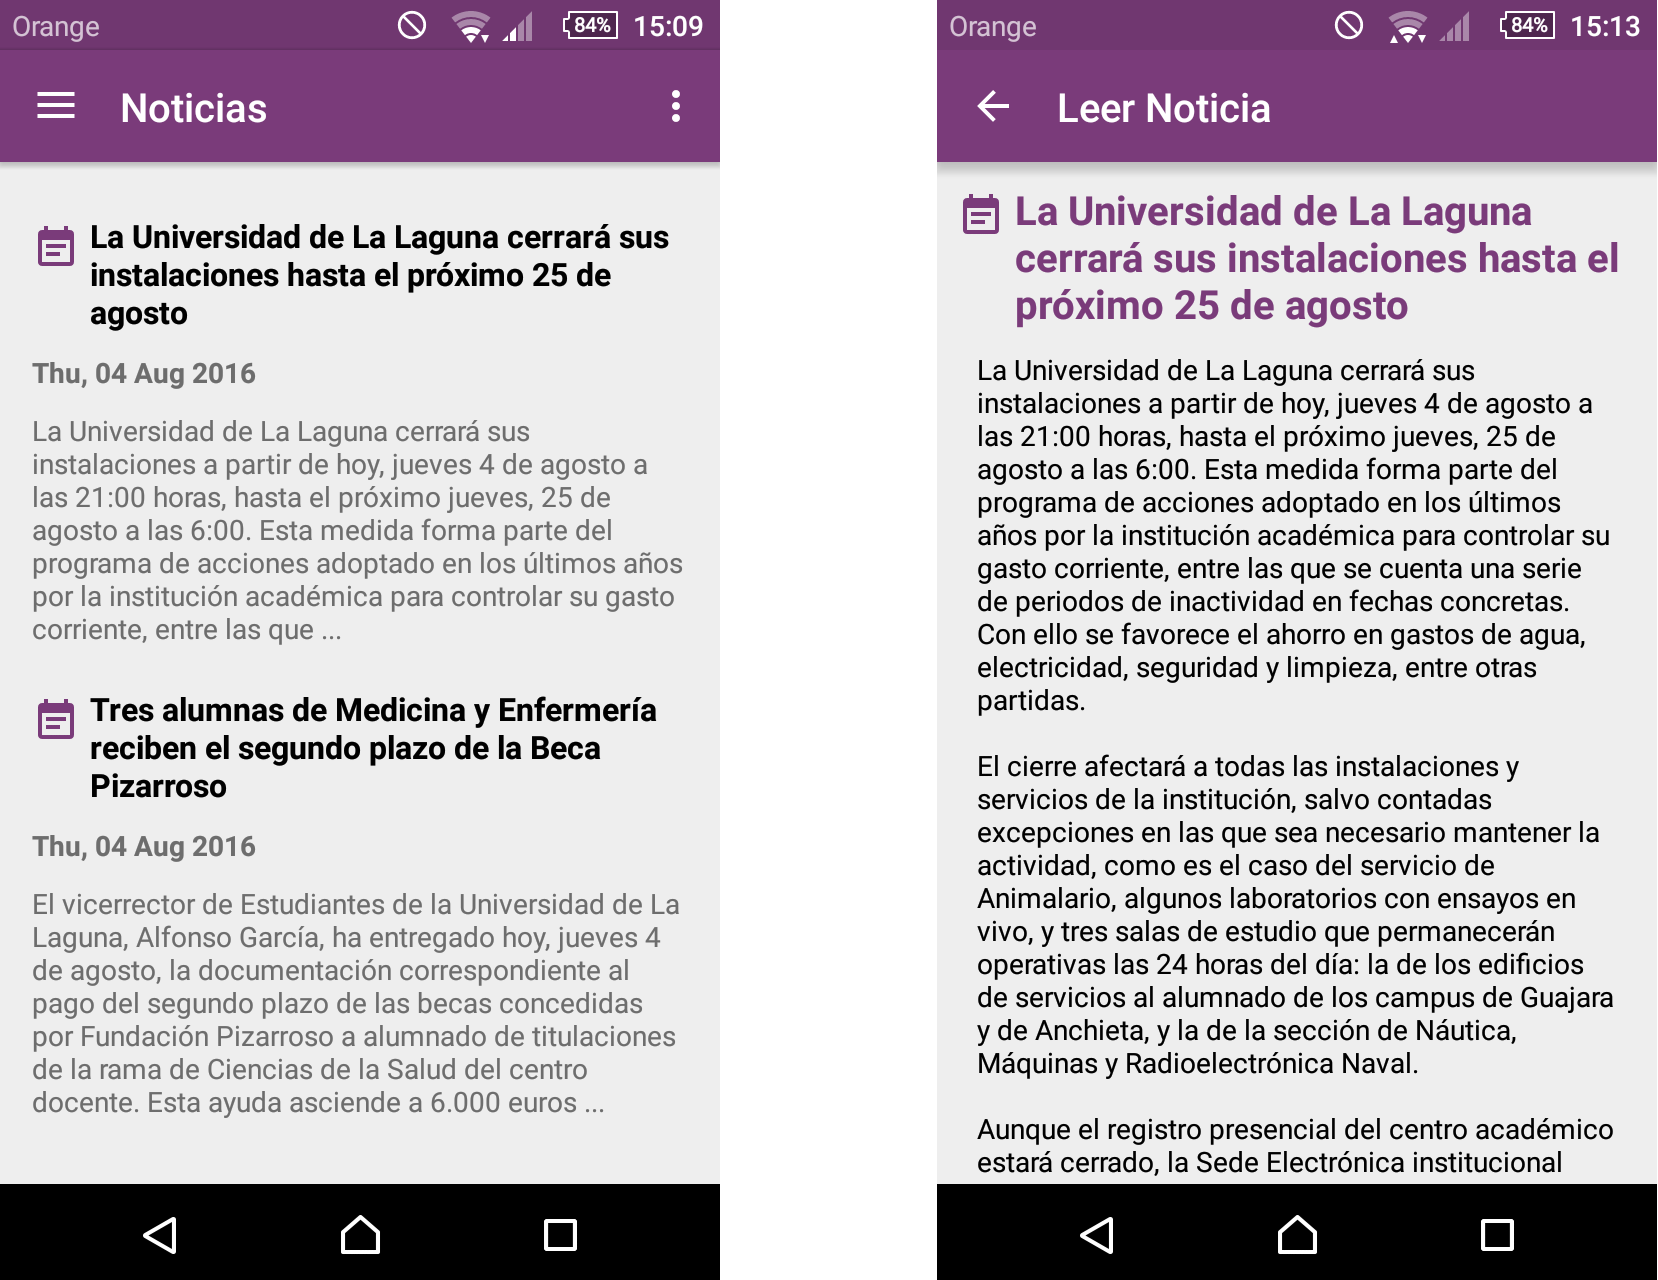
\includegraphics[width=1.0\columnwidth]{noticias.png}
	\caption{Fragmento de Noticias y Actividad de Leer Noticia}
	\label{fig:ejemplo}
\end{figure}

\subsection{Actividad de Reserva}

Los elementos que se muestran en la sección de servicio son seleccionables. El 
usuario puede interactuar con cualquiera de las pistas mostradas para dar paso 
a la operación de reserva. 

Una vez un elemento es seleccionado se inicia la actividad de reserva. Se muestra 
la información de la pista (nombre y tipo de pista), un calendario para que el 
usuario seleccione una fecha y un botón para realizar la acción de reserva. Si 
el usuario decide presionar el botón para reservar la pista, se muestra un 
diálogo para que confirme la acción. Las fechas que no están disponibles se 
muestran en rojo. Si el usuario decide realizar la reserva en una fecha que no 
esté disponible, no se le permitirá reservar y se le mostrará un mensaje de error 
indicando que la cancha ya está reservada para ese día.

La barra de acción cambia. La acción de configuración y el menú de navegación 
desaparecen para solo dar la opción al usuario de ir atrás o realizar la reserva.

\begin{figure}[h]
	\centering
	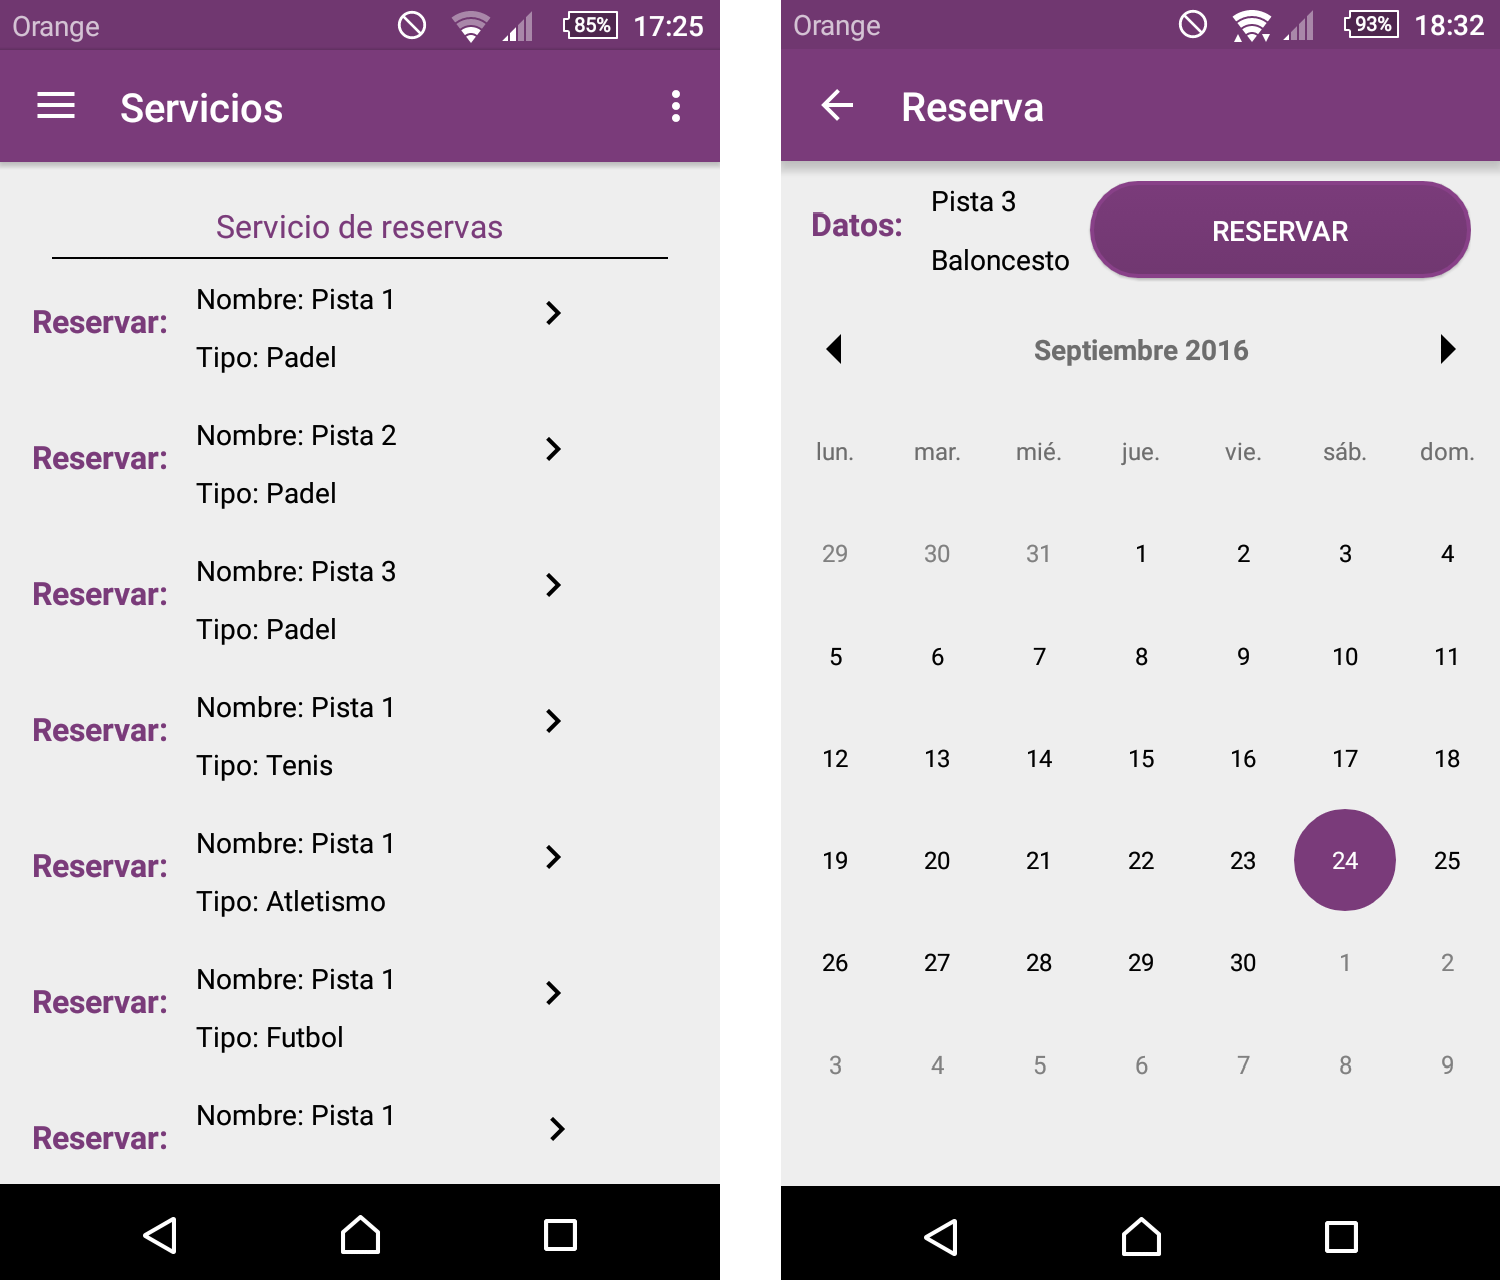
\includegraphics[width=0.7\columnwidth]{servicio.png}
	\caption{Fragmento de Servicios y Actividad de Reserva}
	\label{fig:ejemplo}
\end{figure}

\subsection{Actividad de Mapas}

En esta actividad se muestran ciertos puntos de interés que tienen que ver con la 
universidad, asi como: facultades, comedores o zonas de aparcamiento. Los puntos 
de interés se muestran a través de una serie de marcadores, seleccionables, que 
muestran una breve descripción del punto de interés. 

El mapa es completamente navegable, el usuario puede hacer zoom para acercar o 
alejar el mapa según lo desee.

Además, al seleccionar un marcador, el usuario tiene varios opciones:
la posibilidad de abrir el punto de interés en la aplicación oficial de 
Google Maps, lo cual le permite acceder a más información que ofrece la misma y, 
obtener la ruta hasta la ubicación del marcador, con todas las opciones que 
Google Maps ofrece: distintos medios de transporte, indicaciones, etc.

\begin{figure}[h]
	\centering
	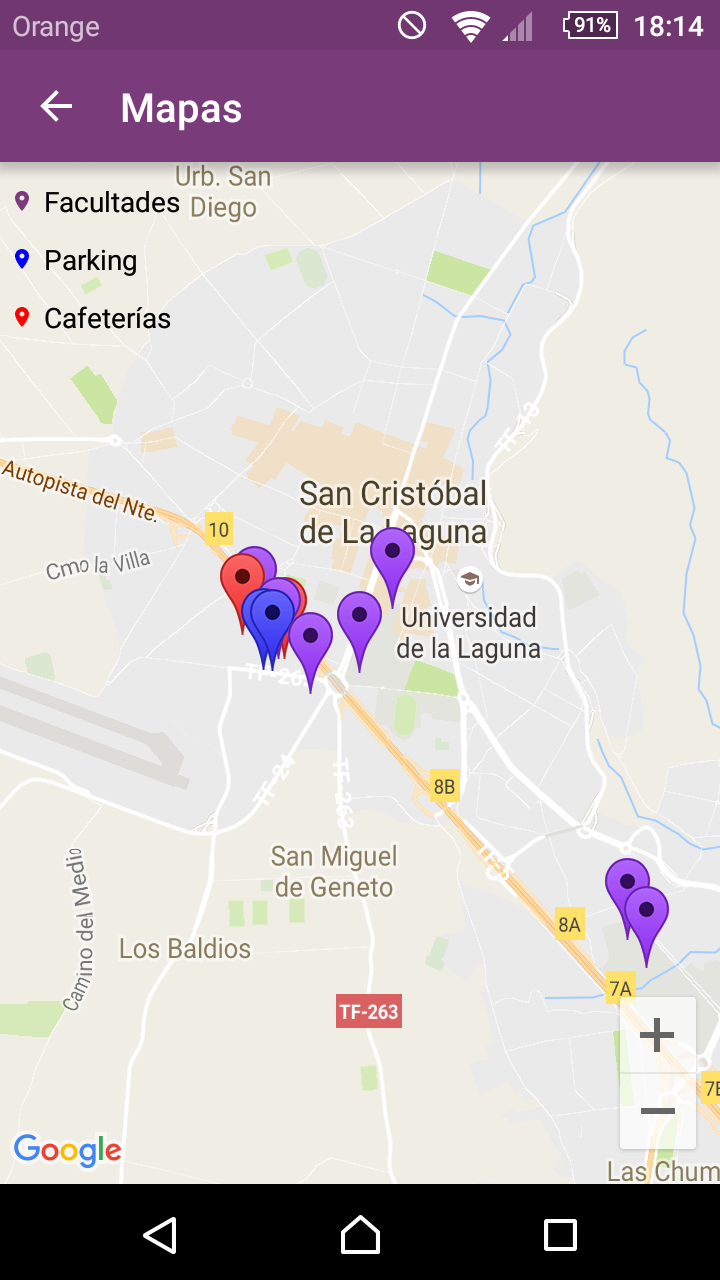
\includegraphics[width=0.4\columnwidth]{maps.png}
	\caption{Actividad de mapas}
	\label{fig:ejemplo}
\end{figure}